\documentclass[]{tufte-book}

% ams
\usepackage{amssymb,amsmath}

\usepackage{ifxetex,ifluatex}
\usepackage{fixltx2e} % provides \textsubscript
\ifnum 0\ifxetex 1\fi\ifluatex 1\fi=0 % if pdftex
  \usepackage[T1]{fontenc}
  \usepackage[utf8]{inputenc}
\else % if luatex or xelatex
  \makeatletter
  \@ifpackageloaded{fontspec}{}{\usepackage{fontspec}}
  \makeatother
  \defaultfontfeatures{Ligatures=TeX,Scale=MatchLowercase}
  \makeatletter
  \@ifpackageloaded{soul}{
     \renewcommand\allcapsspacing[1]{{\addfontfeature{LetterSpace=15}#1}}
     \renewcommand\smallcapsspacing[1]{{\addfontfeature{LetterSpace=10}#1}}
   }{}
  \makeatother

\fi

% graphix
\usepackage{graphicx}
\setkeys{Gin}{width=\linewidth,totalheight=\textheight,keepaspectratio}

% booktabs
\usepackage{booktabs}

% url
\usepackage{url}

% hyperref
\usepackage{hyperref}

% units.
\usepackage{units}


\setcounter{secnumdepth}{-1}

% citations
\usepackage{natbib}
\bibliographystyle{plainnat}


% pandoc syntax highlighting

% table with pandoc

% multiplecol
\usepackage{multicol}

% strikeout
\usepackage[normalem]{ulem}

% morefloats
\usepackage{morefloats}


% tightlist macro required by pandoc >= 1.14
\providecommand{\tightlist}{%
  \setlength{\itemsep}{0pt}\setlength{\parskip}{0pt}}

% title / author / date
\title[Appunti di Fisica Nucleare e Subnucleare]{Appunti di Fisica
Nucleare e Subnucleare}
\author{Niccolò Zanotti}
\date{2022-10-06}

\usepackage{amsmath}
\usepackage{amssymb}
\usepackage{amsthm}
\usepackage{graphicx}
\usepackage{cancel}
% \usepackage[svgnames]{xcolor}
\usepackage[italian]{babel}
\usepackage{bm}
\usepackage{simplewick}
\usepackage{listings}
\usepackage[displaymath,textmath,sections,graphics,floats]{preview}
\usepackage{longtable}
\usepackage{relsize}

\usepackage{pgfplots}
\usetikzlibrary{intersections}
\usetikzlibrary{calc,patterns,angles,quotes}
\usepackage{tikz}
\usepackage{caption}
\usepackage{tikz-network}
\usepackage{float}
\floatplacement{figure}{H}
\pgfplotsset{compat = newest}

\theoremstyle{definition}
\newtheorem{definition}{Definition}

\theoremstyle{theorem}
\newtheorem{theorem}{Theorem}
\theoremstyle{plain}

\theoremstyle{remark}
\newtheorem*{remark}{Remark}

\theoremstyle{remark}
\newtheorem*{example}{Example}

% alias for planck constant
\newcommand{\hp}{\hslash}

% command to insert nuclear element \nucl{A}{Z}{elelement symbol}
\newcommand{\nucl}[3]{ \ensuremath{ \phantom{\ensuremath{^{#1}_{#2}}} \llap{\ensuremath{^{#1}}} \llap{\ensuremath{_{\rule{0pt}{.75em}#2}}} \mbox{#3} } }


\begin{document}

\maketitle



{
\setcounter{tocdepth}{1}
\tableofcontents
}

\hypertarget{lo-studio-del-nucleo}{%
\chapter{Lo studio del nucleo}\label{lo-studio-del-nucleo}}

\hypertarget{la-sezione-durto}{%
\section{La sezione d'urto}\label{la-sezione-durto}}

In quale modo i fisici possono esplorare la struttura di oggetti così
piccoli quali sono gli atomi, i nuclei e le particelle subatomiche?
Quali sono le grandezze fisiche sperimentalmente misurabili e quale tipo
di informazioni su tali oggetti microscopici è effettivamente possibile
ottenere da tali misure?

Gli elementi fondamentali che caratterizzano l'esperimento di
Rutherford(1909-1913) cosí come versioni più moderne sono i seguenti:

\begin{marginfigure}
\texttt{L\textquotesingle{}esperimento\ di\ Geiger-Mursden-\ Rutherford}
\end{marginfigure}

\begin{enumerate}
\def\labelenumi{\arabic{enumi}.}
\tightlist
\item
  un \textbf{fascio incidente} di particelle proiettile;
\item
  un \textbf{bersaglio} contenente le particelle da
  studiare(atomi/nuclei /protoni/neutroni);
\item
  un \textbf{rivelatore} dietro/attorno al bersaglio capace di misurare
  le particelle emergenti\footnote{Il progresso tecnologico nel campo
    delle macchine acceleratrici ha reso possibile una variante dello
    schema descritto dove la collisione avviene tra le particelle di due
    fasci contrapposti. I `collider', certamente più difficili da
    costruire permettono però di raggiungere, a parità delle tecnologie
    di accelerazione delle particelle, una maggiore energia della
    collisione.}.
\end{enumerate}

Nell'esperimento di Rutherford:

\begin{itemize}
\tightlist
\item
  fascio: particelle \(\alpha\) di \(5.6 MeV\)
\item
  bersaglio: gold foil con spessore di \(8.6 \times 10^{-6}\) cm
\item
  rivelatore: vetro dipinto da \(ZnS\) scintillante al momento
  dell'incontro con particelle cariche.
\end{itemize}

\textbf{Goal} dell'esperimento: riconoscere le particelle emergenti e
misurarne le grandezze cinematiche(energia, quantità di moto) al fine di
ottenere informazioni sulla natura dell' \textbf{interazione} tra
particella del fascio e particella del bersaglio.

Il termine \textbf{interazione} è un termine generico. Introduciamo la
seguente notazione:

\begin{itemize}
\tightlist
\item
  \textbf{Processi di diffusione}: particelle emergenti dal bersaglio
  coincidono con quelle del raggio incidente
\item
  \textbf{Processi di produzione}: non vale quanto sopra
\end{itemize}

Tra i processi di diffusione si distinguono processi

\begin{itemize}
\tightlist
\item
  elastici : energia della particella incidente \(=\) emergente
\item
  anelastici: energia della particella incidente \(\neq\) emergente
\end{itemize}

Dato che solitamente la particella proiettile è priva di struttura
interna, a differenza di quella bersaglio, si ha diffusione

\begin{itemize}
\item
  elastica: il bersaglio non modifica la sua struttura e non assorbe
  energia
\item
  anelastica: il bersaglio modifica la sua struttura e assorbe energia
\end{itemize}

Si parla di \emph{diffusione profondamente inelastica} quando l'energia
della particella proiettile è tale che la De Broglie wavelength
associata risulta molto minore della dimensione della particella
bersaglio \(\rightarrow\) si può definirne la struttura interna(che
varia durante il processo).

Sulla base di questa terminologia è evidente che \textbf{un processo di
produzione è sempre inelastico}.

\begin{marginfigure}
\begin{figure}
\centering
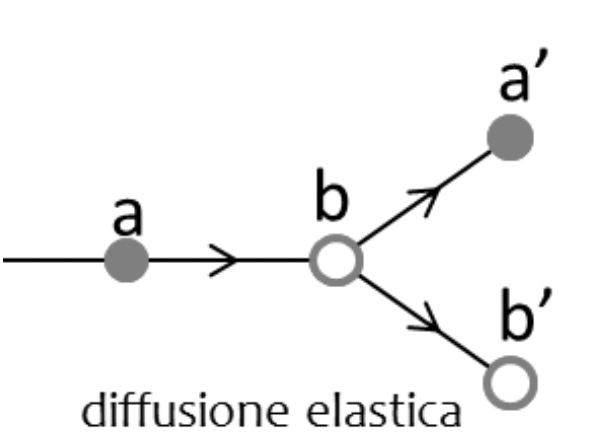
\includegraphics{../figs/diffusione-elastica.jpg}
\caption{alt tex}
\end{figure}
\end{marginfigure}

\bibliography{bibliography.bib}



\end{document}
